\chapter{Cronograma e Gestão de Pessoas}
\label{cap:05}

O planejamento compreende a consolidação do pré-projeto e a elaboração da V0 até novembro de 2026, seguidas pelo desenvolvimento, avaliação e entrega da V1 até junho de 2027. A V0 terá como objetivo verificar a viabilidade técnica do fluxo central, enquanto a V1 constituirá o Produto Mínimo Viável e o compromisso de entrega do trabalho.

Os períodos apresentados são estimativas de planejamento e poderão ser ajustados conforme a disponibilidade da equipe, os resultados dos incrementos e o calendário acadêmico. A data específica da banca técnica da disciplina GPD2 será incorporada quando estiver disponível.

\section{Gestão de Pessoas}

A equipe é composta por Gustavo da Silva Coelho e Raissa Carla Ferreira da Silva. Gustavo concentrará sua atuação no desenvolvimento e na integração técnica, com disponibilidade de até seis horas semanais. Suas responsabilidades principais serão a implementação do backend em Python e FastAPI, a integração com PostgreSQL e com o modelo de linguagem, a construção da interface em React e o empacotamento com Electron, além dos testes técnicos e da correção de falhas.

Raissa concentrará sua atuação na organização do cronograma, acompanhamento das atividades, consolidação da documentação e preparação da apresentação, com disponibilidade estimada entre seis e oito horas semanais. Também apoiará a organização das evidências de avaliação e a comunicação da proposta, de suas contribuições e dos resultados obtidos.

A divisão representa a concentração principal das atividades, sem impedir a colaboração entre os integrantes. Ambos participarão das decisões de escopo e arquitetura, da definição das perguntas de avaliação, da conferência dos resultados esperados, da revisão do relatório e da preparação da defesa.

O projeto contará com a orientação do professor Giovani Fonseca Ravagnani Disperati. Os encontros com o orientador serão acordados conforme sua disponibilidade e os marcos do projeto. A avaliação acadêmica envolverá o orientador e os professores responsáveis pelas etapas do trabalho.

O acompanhamento será realizado por meio de um processo baseado em Kanban, com backlog priorizado e reuniões semanais entre os integrantes. As tarefas deverão indicar responsável, resultado esperado e situação, utilizando estados como a fazer, em andamento, em revisão e concluída. O código-fonte será versionado com Git e mantido no GitHub. A documentação e os testes acompanharão o desenvolvimento.

\section{Cronograma das Atividades}

A Figura~\ref{fig:cronograma-projeto} apresenta as atividades previstas até a Avaliação Final do Projeto Integrador. As linhas numeradas correspondem às descrições apresentadas a seguir. Cada marcação \textbf{X} indica o mês previsto de realização, sem representar uma atividade já concluída.

\FloatBarrier
\begin{figure}[!htbp]
    \centering
    \caption{Cronograma previsto de outubro de 2026 a junho de 2027}
    \label{fig:cronograma-projeto}
    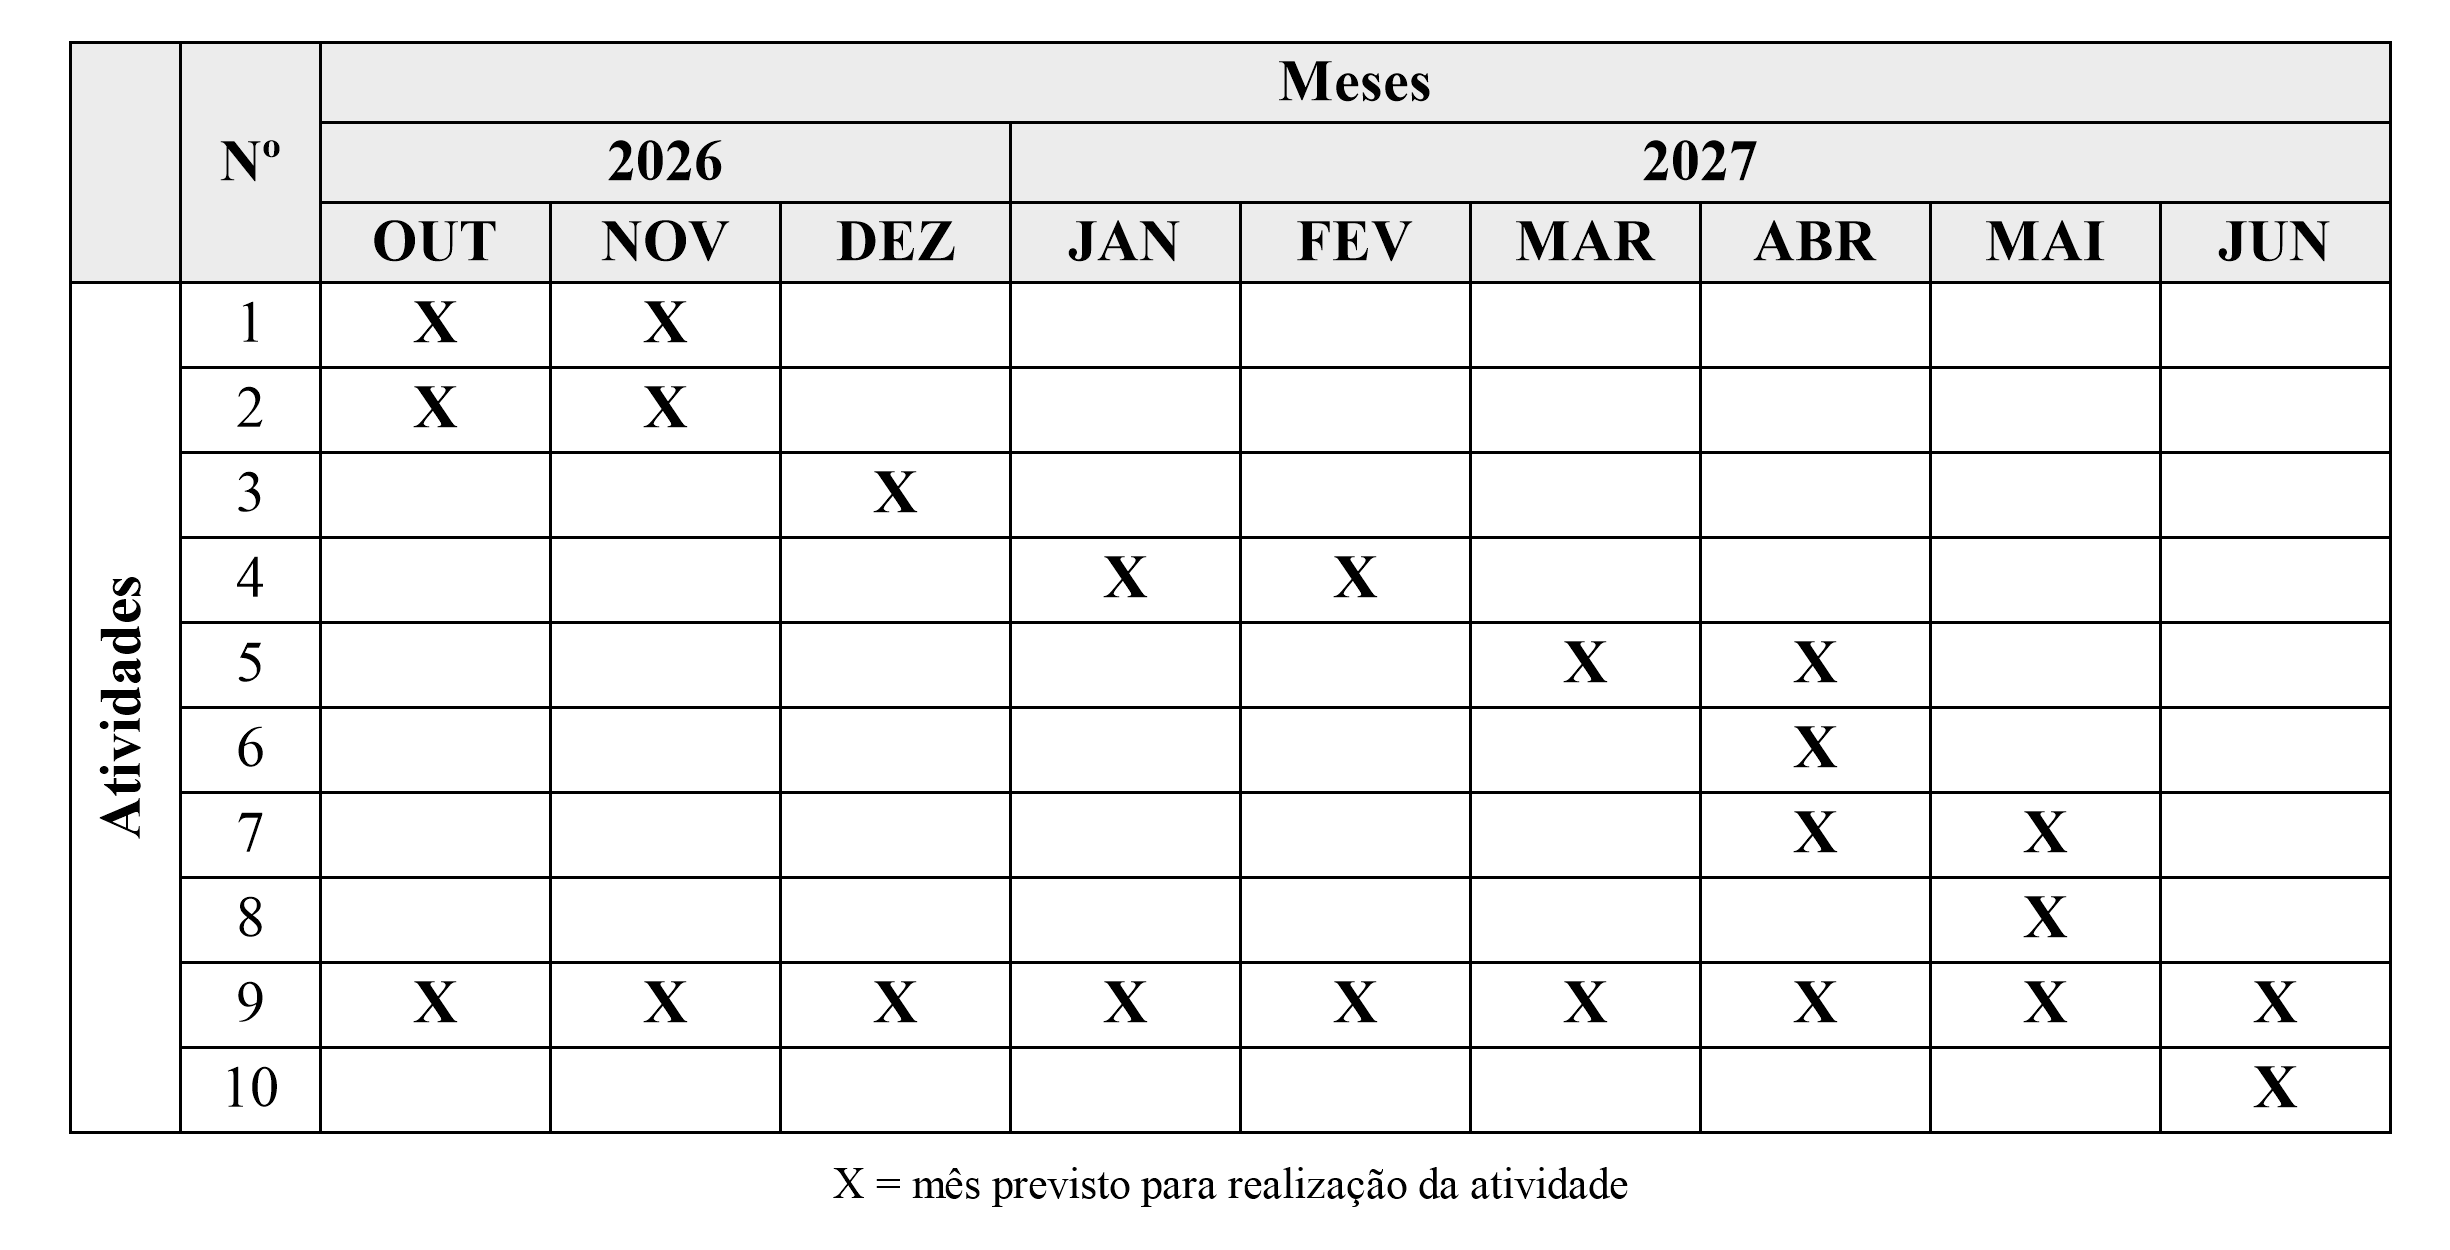
\includegraphics[width=\textwidth]{imagens/cronograma}
    \par\smallskip
    {\footnotesize Fonte: Elaborado pelos autores (2026).}
\end{figure}
\FloatBarrier

\begin{enumerate}
    \item \textbf{Consolidação do pré-projeto (outubro e novembro de 2026):} uniformizar escopo, requisitos, tecnologias, modelos e conclusões parciais, além de registrar o planejamento da equipe e da avaliação.

    \item \textbf{Desenvolvimento da V0 (outubro e novembro de 2026):} implementar uma prova de conceito de conexão com PostgreSQL, introspecção, preparação de contexto, geração, validação e execução de consultas. Incluir consentimento binário para amostras de até cem registros por tabela, com todas as colunas, e utilizar inicialmente um subconjunto de perguntas de teste.

    \item \textbf{Revisão da V0 e planejamento da V1 (dezembro de 2026):} analisar os resultados iniciais, identificar pendências técnicas, apoiar a escolha do modelo e do provedor de linguagem e organizar o backlog e o fluxo da interface.

    \item \textbf{Desenvolvimento do núcleo da V1 (janeiro e fevereiro de 2027):} integrar conexão, consentimento, contexto, geração de SQL, validação, execução com credenciais de leitura, tratamento de falhas e registro das informações de execução. O fluxo admitirá três tentativas totais, incluindo a inicial.

    \item \textbf{Interface e integração desktop (março e abril de 2027):} desenvolver e integrar a interface com React, Vite e TypeScript, disponibilizando conexão, perguntas e resultados tabulares, e organizar a execução local com Electron e backend em FastAPI.

    \item \textbf{Preparação da avaliação (abril de 2027):} consolidar o banco comercial fictício, as perguntas, as consultas de referência, os resultados esperados e os casos de segurança e falha. Congelar os dados e as amostras utilizados na comparação final.

    \item \textbf{Estabilização e correções da V1 (abril e maio de 2027):} verificar os requisitos obrigatórios, executar testes de integração e corrigir os problemas identificados no fluxo principal e na avaliação.

    \item \textbf{Avaliação comparativa e análise dos resultados (maio de 2027):} executar as perguntas com esquema e com esquema acrescido de amostras, registrar métricas e analisar respostas incorretas, tentativas de correção, custos e limitações.

    \item \textbf{Documentação e acompanhamento (outubro de 2026 a junho de 2027):} atualizar o relatório, as decisões, o backlog, os registros de teste e as evidências do trabalho, com participação dos dois integrantes e maior concentração de Raissa na organização documental.

    \item \textbf{Apresentação e entrega final (junho de 2027):} concluir a discussão dos resultados, revisar o relatório e a V1, preparar os materiais de apresentação e realizar a entrega para avaliação final.
\end{enumerate}

A integração e a conclusão dos requisitos essenciais serão priorizadas antes da etapa final. Maio será reservado principalmente para avaliação e correções, enquanto junho será destinado à consolidação da entrega e à apresentação. As versões V2 e V3 permanecerão como possibilidades de evolução, sem integrar o compromisso obrigatório do cronograma.

\section{Planejamento da Avaliação}

A avaliação técnica será conduzida pelos autores em um banco PostgreSQL fictício do domínio comercial, contendo clientes, produtos, pedidos e itens de pedido. Será preparado um conjunto de trinta perguntas válidas em português, distribuídas entre dez consultas simples, oito agregações, oito consultas com junções e quatro consultas que envolvam significado de negócio. Adicionalmente, serão propostas dez verificações de solicitações proibidas e cinco verificações de falhas operacionais.

Cada pergunta válida terá sua interpretação esperada, uma consulta SQL de referência e o resultado esperado documentados. As perguntas utilizadas para ajustes durante o desenvolvimento serão separadas das utilizadas na avaliação final. O banco incluirá situações que permitam identificar erros, como pedidos cancelados, valores nulos e registros próximos aos limites dos períodos consultados.

Uma resposta será considerada correta quando os dados retornados corresponderem ao resultado esperado, incluindo filtros, valores, agrupamentos e ordenação quando solicitada. A igualdade textual com o SQL de referência não será exigida. Consultas que executem sem erro, mas respondam a uma intenção diferente, serão classificadas como incorretas.

O efeito das amostras será investigado pela comparação entre duas configurações:
\begin{enumerate}
    \item contexto contendo apenas os metadados estruturais do banco;
    \item contexto contendo os mesmos metadados e amostras autorizadas de até cem registros por tabela, incluindo todas as colunas.
\end{enumerate}

O modelo, as instruções, as perguntas, os dados e a política de correção serão mantidos constantes. As amostras serão fixadas para permitir a reprodução da comparação. Prevê-se realizar três execuções por pergunta em cada configuração, totalizando cento e oitenta execuções de solicitações válidas, além das verificações de segurança e falha. Cada execução respeitará o limite de três tentativas totais.

Serão registradas a taxa de respostas corretas na primeira tentativa e após as correções, a taxa de execução SQL bem-sucedida, a quantidade de tentativas, a latência e, quando disponíveis, o consumo de tokens e o custo estimado. Os resultados serão apresentados por configuração e grupo de perguntas. Os casos de segurança e falha serão contabilizados separadamente.

Como metas preliminares para discussão com o orientador, propõem-se:
\begin{itemize}
    \item pelo menos 80\% de respostas corretas às perguntas válidas na configuração com amostras, considerando até três tentativas totais;
    \item pelo menos 90\% de solicitações válidas com execução SQL bem-sucedida nessa configuração, independentemente da correção semântica;
    \item nenhuma alteração do banco nas dez verificações de solicitações proibidas;
    \item encerramento controlado nas cinco verificações de falhas operacionais;
    \item ausência de envio de registros ao modelo quando o consentimento for recusado;
    \item realização do fluxo principal pela interface gráfica, sem utilização de terminal pelo usuário.
\end{itemize}

Essas metas deverão ser revisadas com o orientador antes da avaliação final e não constituem critérios oficiais da banca. A configuração sem amostras será avaliada separadamente, sem pressupor que a inclusão de registros necessariamente melhore o desempenho. A meta de latência e os limites de custo serão definidos após as medições da V0.

A avaliação pelos professores considerará a coerência da proposta, a demonstração do sistema, a documentação e as evidências apresentadas. Essa participação não será tratada como um estudo de usabilidade com usuários finais.

% Orientação do template: manter este capítulo em GPD1 e GPD2.
% Para a versão da banca final, removê-lo ou transferi-lo para um apêndice.

